% !TeX root = ../main.tex
% Add the above to each chapter to make compiling the PDF easier in some editors.

\chapter{Fast-Relays}\label{chap:fast_relays}

In this chapter we will dive into the specifics of our proposed fast-relay setup.
We will cover necessary adaptations as well as setup specifics like eBPF programs 
and userspace synchronization.
Figure~\ref{fig:route-layering} already shows a high level overview of a basic 
server-relay-client setup with its respective networking layers.
A conventional setup would have the packet travel into userspace at the relay
while our setup aims to reduce the critical path, as is indicated using the red arrows.

\vspace{0.5cm}
\begin{figure}[htbp] % TODO: where to put this?
    \centering
    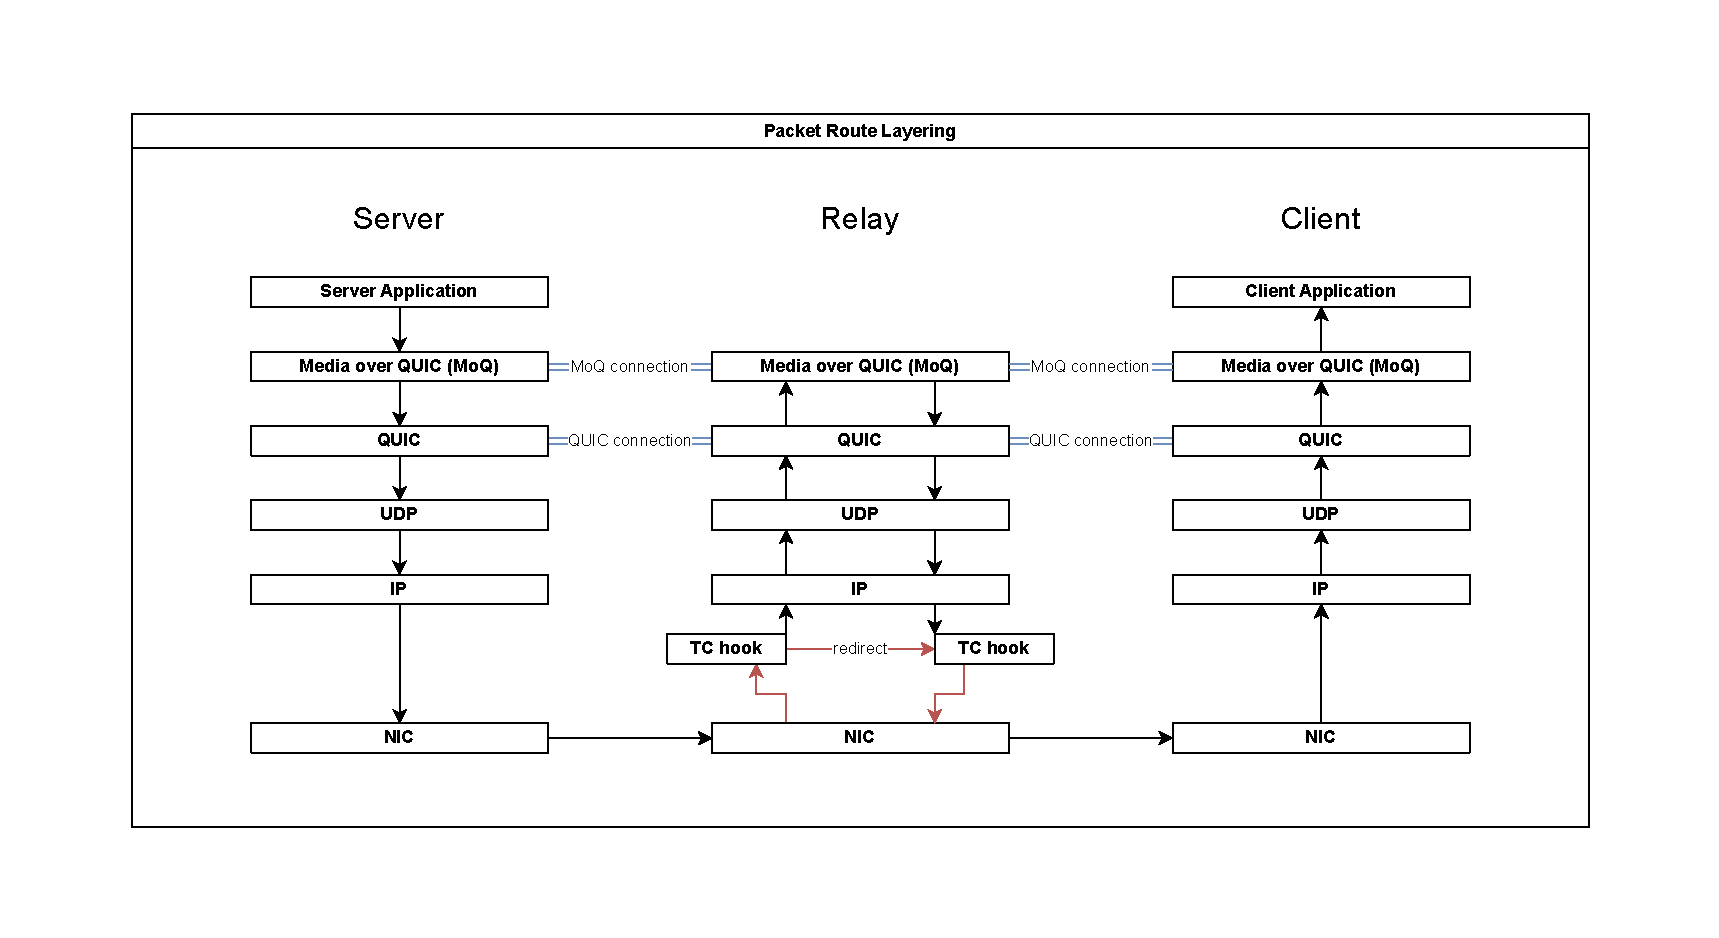
\includegraphics[width=0.7\textwidth]{figures/02_background/route-layering.drawio.pdf}
    \caption[Packet path schematic regarding network stack]{Conventional networking layers a packet passes.
    The red loop indicates again the ``short-cut'' that is utilized by the fast-relay 
    (eBPF packet-forwarding {-} no need to go up to userspace).}\label{fig:route-layering}
\end{figure}

\section{QUIC Adaptions}\label{sec:quic_adaptions}
As was already mentioned in the previous chapter, our setup requires some adaptations
to the quic-go library.
One initial change necessary was to turn off packet en- and decryption, 
that is happening within quic-go.
Given that we operate on the QUIC-header data within the eBPF program, we need access 
to fields that are encrypted using QUIC header-protection.
For obvious reasons sending unencrypted packets is not something that would be wanted in 
a production environment, but for our exemplary setup, it is unproblematic. 
An alternative would be to ``push down'' en- and decryption onto a smartNIC using a 
hardware offload, but at the time of writing, there was no such offload available for QUIC\@. 
Given that such a hardware offload is added in the future, the en- and decryption can be
turned on again, which makes this change more of a temporary solution to show the feasibility
of our approach.

\subsection{Function-Pointer Style Additions}
Another type of change that we needed to introduce into the quic-go library is caused by 
connection state management.
We essentially added support for communication with the eBPF program by using an 
approach similar to C-style function pointers.

On multiple locations, we added conditional function calls like the one depicted in 
\autoref{changes:function-pointer}.
The function that is called here will be defined by the developer of the relay and 
therefore allow for customizability without the need for changing the library itself.

\vspace{0.5cm}
\noindent\begin{minipage}{\textwidth}
\begin{lstlisting}[style=GoStyle, label=changes:function-pointer, caption=An example of a function-pointer addition to the quic-go library.]
    /* Function pointer call within actual quic-go code */
    if packet_setting.ConnectionUpdateBPFHandler != nil /* && potentially other conditions */ {
	    packet_setting.ConnectionUpdateBPFHandler(connId.Bytes(), uint8(connId.Len()), p.connection)
	}
\end{lstlisting}
\end{minipage}

\vspace{0.5cm}
\noindent\begin{minipage}{\textwidth}
\begin{lstlisting}[style=GoStyle, label=changes:signature-function-pointer, caption=Only the signature will be defined within the library itself.]
    /* Function pointer signature definition within additional config file */
	ConnectionUpdateBPFHandler      func(id []byte, l uint8, conn QuicConnection) = nil
\end{lstlisting}
\end{minipage}

The definition of the function that the developer of the relay wishes to be executed at specifically
defined points will be defined locally in the relay code and provided to the configuration of the quic-go library.
An example of how this could look like is shown in \autoref{changes:definition-function-pointer}.

\vspace{0.5cm}
\noindent\begin{minipage}{\textwidth}
\begin{lstlisting}[style=GoStyle, label=changes:definition-function-pointer, caption=An example of how the addition looks on the relay side.]
    /* Definition of the function within the local relay code */
    func localUpdateConnectionId(id []byte, l uint8, conn packet_setting.QuicConnection) {
        /* handle the connection update by interacting with the eBPF program */
    }   

    /* Providing the function to the quic-go library */
    func main() {
        /* ... */
        packet_setting.ConnectionUpdateBPFHandler = localUpdateConnectionId
        /* ... */
    }
\end{lstlisting}
\end{minipage}

The need for these additions arises since the eBPF program works with its own copy of the current state of a connection.
This, for example, includes the connection-id that will be used when changing the packet header before sending it out.
Since a connection-id can change, i.e.~be updated or retired, during the lifetime of a connection, we need a way to inform 
the eBPF program to no longer use outdated state-information.
These function-pointer style additions provide a minimal way of adding such functionality without limiting flexibility 
or adding too much application-specific code to the library itself, as would be the case if the library would access 
the eBPF-Maps directly.

% TODO: mention changes which are not function-pointer style
\subsection{Direct Changes to the Library}

\iffalse
% open stream with priority (+ datagram)

% turn off crypto (reaction to CRYPTO_TURNED_OFF flag)

% connection-id retirement specific stuff (switch to priority id)

% fixed sizes for fields e.g. conn id, stream-id, etc.(just for ease of development)

% e.g. only single stream frame inside packet (for ease of development) since general approach too complex for verifier?

% retransmission functions that open new stream with correct id

% registerBPFPacket function for connection

% prio enum. (prolly could be also given by relay dev) % TODO: not interessting enough i'd say
\fi

Besides the simple function-pointer style additions, we also had to make some direct changes to the library.
These include simplifications of the packet structure to make the implementation of a prototype easier 
but also changes that are necessary for the whole approach to work.
The necessary state changes mainly required internal state adjustments that would not be possible from outside 
the library because of missing access/visibility.
The optional turn-off for the packet en- and decryption based on the value of the \verb|CRYPTO_TURNED_OFF| flag
also required some direct changes to the library, but these will not be mentioned further since they are temporary
and not a focus of this chapter.

\subsubsection*{Simplifications of Packet Structure}
We added some changes to the quic-go library to make a prototype implementation easier.
The first one is that we fixed the sizes of some variable length fields like the connection-id or the stream-id.
This was mainly to avoid the need to figure out the correct sizes within the eBPF program as this would have 
resulted in approaches that would have to be very carefully turned into eBPF-compatible code due to verifier
restrictions.
Besides fixing the length of some fields, we also limit the number of frames per packet to one.
Normally a QUIC packet can contain multiple frames, especially stream-frames, but this would have required 
a packet traversal within the eBPF program that, again, would have been harder to implement considering all
verification constrictions.
Besides this additional complexity, for our usecase the ``singe-stream-frame-per-packet'' approach is not changing
a lot since the payload of one media packet will be split into multiple packets due to its size.
This means a single stream frame is likely already using up a whole packet, and multiple frames per packet would 
not be happening.

\subsubsection*{Stream Priorities}
Our approach relies on the fact that every packet has a priority value assigned to it.
In our case this priority value is stored within the connection-id.
Based on this, the first change, which is not only for simplification of our prototype implementation but is actually needed for 
our approach to work, is the addition of opening a stream with a specific priority.
Our assumptions define that the server is the one marking the packets with the correct priority, which in 
our case is realized by sending them over a specific stream.
Every stream is bound to a specific priority value, and our code changes will make sure that the connection-id
that is used for any packet sent on this stream will contain the correct priority value.
Figure~\ref{fig:priority-stream} visualizes the setup as well as our rudimentary approach of saving the 
priority value as the first byte of the connection-id.

\vspace{0.5cm}
\begin{figure}[H]
    \centering
    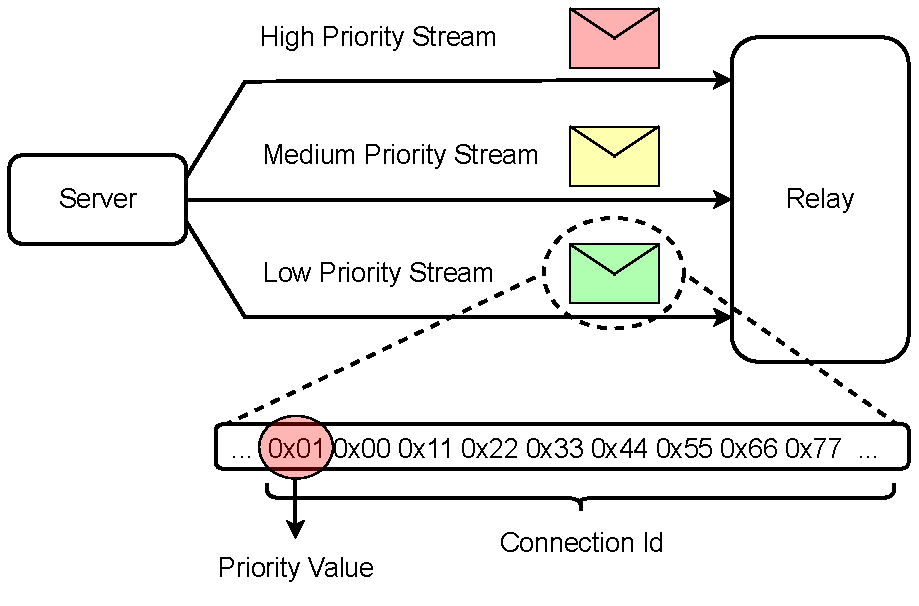
\includegraphics[width=0.7\textwidth]{figures/03_fast_relays/priority-streams.drawio.pdf}
    \caption[Streams with specific priorities]{The server opens streams with specific priorities, 
    which are then used to send packets with the corresponding priority.}\label{fig:priority-stream}
\end{figure}

This approach of having the priority value saved within the connection-id caused the need for another 
change in the library.
Due to the periodic change/retirement of connection-ids, we need to make sure that at any point in time, there 
exists one connection-id for each priority within the connection.
Otherwise, we might be unable to mark a packet with the correct priority.
This led us to introduce some additional logic to the code that is executing the retirement of connection-ids.
There, we will make sure that before a connection-id is retired, either one with the same priority value
already exists or is created.
This solves the problem of not being able to mark a packet with the correct priority.

\subsubsection*{Retransmission}
Another direct change that is needed is that of a specific \verb|OnLost| function for packets that 
have been forwarded by the eBPF program.
Since the relay state is not necessarily aligned with the server state, and the relay does not know
about the stream a packet was sent on, it is not possible to reuse the plain \verb|OnLost| function
of the quic-go library.
This is because the plain \verb|OnLost| function would lookup the stream corresponding to the provided stream-id and 
retransmit the packet on there, but the stream for the given id might not exist within the relay stream-pool.
Instead, our new function needs to look up the stream-id of the lost packet and open a new stream with
the same stream-id, ensuring that the client correctly receives the retransmission.
Besides the stream-id, the created stream-object should also have the same remaining stream-state
as the original stream (e.g.~offset-information).  
When a retransmission happens, the relay also needs to tell the underlying eBPF program that a packet is part of a 
retransmission and that, even if a stream was actually created by the relay, the egress program should treat it like 
it was created by the server.
That last part is necessary for the stream-id translation part of the egress program, which is explained further
in section\nobreakspace\ref{sec:client-egress}, to work correctly.
This functionality of informing the eBPF program about the retransmission, however, is again realized by a 
function-pointer style addition and thus designed by the relay developer.

\subsubsection*{Visible Endpoint for Packet Registration}
The last direct change that we added was the introduction of an additional function \verb|RegisterBPFPacket| 
on a quic-go connection object that allows the relay to register a packet.
Since the packet registration requires access to internal state of the connection, this also needed to be 
done as an actual change to the library.
Now the relay can just read the necessary information of a packet that needs to be registered
from the eBPF-maps and then pass it on to this function which will handle the registration.
This also provides a good separation between the Go code that handles eBPF communication and the actual
QUIC connection handling.
\section{eBPF Setup}\label{sec:ebpf_setup}
\subsection{Different eBPF Programs}
\begin{figure}[htbp]
    \centering
    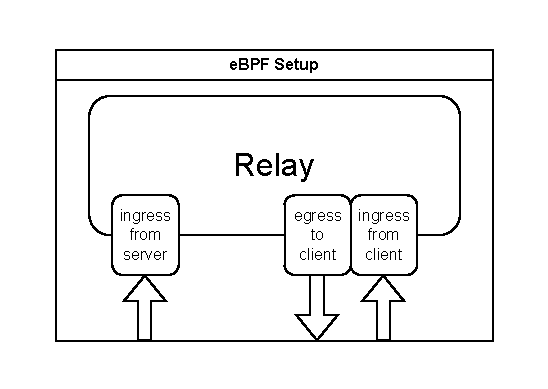
\includegraphics[width=0.3\textwidth]{figures/03_fast_relays/ebpf-setup.drawio.pdf}
    \caption[Types of eBPF programs at relay]{The relay has to be equipped with three BPF programs.}\label{fig:ebpf-programs}
\end{figure}

In order to allow the relay to forward packets independently of the userspace, we
need to equip the relay with three BPF programs as seen in figure.
Those three programs are 
\begin{itemize}
    \item a program that handles incoming traffic \textbf{from} the clients (client ingress),
    \item a program that handles outgoing traffic \textbf{to} the clients (client egress) and
    \item a program that handles incoming traffic \textbf{from} the video server (server ingress).
\end{itemize}
Their responsibilities then are
\begin{itemize}
    \item handling the initial registration of new clients and storing their information such as
    MAC addresses in a BPF map,
    \item intercepting the packets from the video server, duplicating and redirecting them to 
    the egress program (as well as sending one unaltered packet to userspace for state
    management purposes),
    \item receiving the redirected packets at egress, altering them using the client specific
    data, deciding (based on packet priority and client congestion) if a packets should be dropped 
    or sent, storing info on sent out packets for future congestion control purposes and finally sending 
    them out to the clients.
\end{itemize}
This setup allows us to separate any state management and congestion control from the actual
packet forwarding and thus makes leaving out any immediate userspace processing possible.

Following is a more detailed description of the responsibilities of each of the three programs.
\subsubsection{Client Ingress} 
The ingress eBPF program initially does some simple packet inspection on every incoming packet 
looking if the packet uses the correct protocols and addresses the right application layer.
This is done by initially parsing the Ethernet, IP and UDP headers, if present, and checking if 
the port matches the listening port the relay application is listening on.
This means the correct port is to be defined prior such that the eBPF program can associate 
a single or (multiple) relay instance(s) with the correct port.
In our case then, since we use QUIC, the program will check for QUIC long header packets that 
setup an initial connection and saves the transmitted state information such as connection id, 
stream related states, etc.~in an eBPF map together with information that is not directly known
by the userspace such as the MAC address of the client.
Saving data like the MAC address directly once the connection is set up allows to omit any further 
Address Resolution Protocol (ARP) steps later on. 
\subsubsection{Server Ingress}
Another ingress related program, this time for packets coming from the video server, is needed
to handle packet duplication and forwarding.
This program will receive the actual video packets from the server and then, based on an internal 
counter of how many clients actually want to receive the video, duplicate the packet accordingly.
The counter of clients will be updated by the userspace once a new connection is fully established
and the client is ready to receive the actual video data.
This might potentially cause some miniscule delay when updating the counter but sending cached 
video data to the client for a brief moment when updating the counter could be a solution for that. % TODO: needed?
Figure~\ref{fig:packet-forwarding-duplication} shows the packet duplication and forwarding process 
high level for an example setting with three clients that want to receive the video data.
In the ingress program from the server we need to consider a few things to ensure the correctness
of our approach.
These are:
\begin{enumerate}
    \item   The program can \textbf{only} forward packets that containing video data and must not 
            forward any other packets that contain e.g.~control data.
    \begin{enumerate}
        \item   This is fairly easy to achieve by doing some header inspection of the QUIC header
                which contains the packet type. Also since payload is generally sent using 
                0-RTT- (i.e.~short-) headers there is no need to consider long-header packets.
    \end{enumerate}

    \item   The program should pass an unaltered copy up to userspace to allow the QUIC library to
            gain knowledge of the packet and handle any state changes accordingly.
    \begin{enumerate}
        \item   Generally speaking this is not strictly necessary as one could just have a separate 
                setup of registering packets that came from the server but as this is not needed
                it is considerably easier to just pass the packet up to userspace and let the 
                library handle it normally. This does not impose any additional overhead as the
                forwarding of any duplicate packets happens independently of course.
        \item   Any packet that has been identified as not part of our dataflow should of course 
                be passed up to userspace without being forwarded to egress.
    \end{enumerate}
\end{enumerate}

\begin{figure}[htbp]
    \centering
    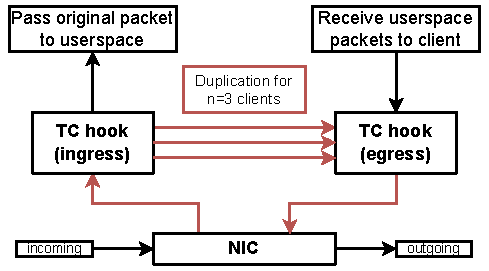
\includegraphics[width=0.5\textwidth]{figures/03_fast_relays/packet-forwarding.drawio.pdf}
    \caption[Video packet duplication]{Duplication and forwarding of video packets to egress directly 
    from ingress.}\label{fig:packet-forwarding-duplication}
\end{figure}

Duplicating and forwarding incoming packets happens using that were identified as payload 
can be done using \verb|bpf_clone_redirect(skb, egress_ifindex, 0)| which is a helper function
that allows one to clone the packet buffer provided as the first argument and add it to the 
queue of the interface that is provided as the second argument.
The last argument allows to specify additional flags.
Aside from \verb|bpf_clone_redirect| there are also other helper functions regarding packet
redirection with slightly different behavior so it is crucial to choose the appropriate one
to get the desired outcome.
Table~\ref{tab:skb-redirection} shows them together with a brief description of their behavior:

\begin{table}[htbp]
    \centering
    \begin{tabular}{L{7cm}L{7cm}}
        \toprule
            Helper & Description \\
        \midrule
            \verb|bpf_clone_redirect| & Clones and redirects a packet to the interface associated with the provided index.\\
        \midrule
            \verb|bpf_redirect| & Redirects a packet to the interface associated with the provided index. The packet is not cloned 
                                    (no underlying call of \verb|skb_clone()|) so it is slightly more efficient (25\% pps increase according 
                                    to commit message). The packet is also not redirected immediately but after the function finishes.\\ % TODO: find commit message
        \midrule
            \verb|bpf_redirect_peer| & Similar to \verb|bpf_redirect| but instead of redirecting the packet to the interface provided 
                                        as a parameter it is redirected to its peer device. This works only between different netns to 
                                        allow for an efficient ``ingress to ingress netns switch''. The switch is more performant since 
                                        the packet does not need to go through the CPU backlog queue.\\ % TODO: what does the CPU backlog queue do?
        \midrule
            \verb|bpf_redirect_neigh| & Again similar to \verb|bpf_redirect| but allows to redirect a packet to another net device. 
                                        This helper does also fill in all the correct L2 addresses of the neighboring subsystem. 
                                        Internally this executes a neighbor lookup to find the needed L2 information. \\
        \bottomrule
    \end{tabular}
    \caption[Redirection helpers for packet buffer]{Helper functions for packet redirection.}\label{tab:skb-redirection}
\end{table}
% TODO: ^^^^^^^^^^^^^^^^^^^^^^^^^^^^^^^^^^^^^^^^^^^^^^^^^^^^^^^^^^^^^^^^^^^
% TODO: cite this: https://man7.org/linux/man-pages/man7/bpf-helpers.7.html
% TODO: cite this: http://arthurchiao.art/blog/differentiate-bpf-redirects/ ???
Based on the descriptions of the redirection helper functions mentioned in table~\ref{tab:skb-redirection}
it becomes clear that \verb|bpf_clone_redirect| is the only suitable for our use case. 
This is becaus we need the cloning aspect since we essentially want to duplicate the incoming packets multiple times.
Also the redirection to another namespace or another net device as provided by \verb|bpf_redirect_peer| and
\verb|bpf_redirect_neigh| respectively is not needed in our case since we operate in the same relay-namespace
throughout the whole process.

\subsubsection{Client Egress}
The central part of the eBPF setup where all the state-management and forwarding of the other 
eBPF programs comes together is the program that handles the outgoing traffic towards the clients.
The client egress program sees every packet that leaves the relay, which includes packets that have 
been redirected by the ingress program as well as packets that have been generated by the relay itself
(i.e.~come from the relay userspace).
This means that the program essentially merges two streams of packets into one stream that needs to 
be in a consistent state.
This interleaving of packets grows the requirements of the program to the following list.
Bold numbers indicate that a requirement is caused by the interleaving of packets.
\begin{enumerate}
    \item[1.]   Obviously, similar to the other eBPF programs any packet that is not part of our traffic 
            should be passed on normally without any further processing.
    \item[\textbf{2.}] In case the packet is QUIC (for the correct client connection) the packet number 
            needs to be changed to a program internal counter to avoid issues of reusing packet numbers. 
            This is the only place where we can guarantee sequential packet numbers since neither 
            userspace nor the server know what the highest packet number sent at any moment in time is. 
            As there is no way of synchronizing lookups (e.g.~using eBPF maps) of information between userspace 
            and eBPF program changing it right before sending it out is the most efficient way. 
    \item[\textbf{3.}] In case the packet (additionally to being QUIC for a client connection) contains 
                        stream frames we need to do a similar translation of the stream id.
                        Reasons and methods for this are the same as for the packet number translation.
                        Figure~\ref{fig:stream-id-translation} shows a flow diagram of the stream id translation
                        process.
                        Important steps include checking if the stream id translation is already existing as well
                        as checking if the packet is a retransmission.
                        The former is necessary in case a payload is split into multiple packets and the latter is 
                        necessary since the retransmission physically come from the relay but should be treated as 
                        if they came from the server.
    \item[4.] Again in case the packet is QUIC and for the right connection the program needs 
                        to read the priority of the packet and decide via map-lookup if the connection 
                        allows for sending packets with the given priority.
    \item[5.] In case the packet is a redirected media stream data packet the program needs to find out 
            which client is the receiver. 
            This is done by saving the client id in some part of the packet that will be overwritten 
            at egress (namely the connection id) before redirecting the packet.
            The egress program, knowing where the id is saved in case of a redirected packet, can then
            lookup the correct address data of the client (i.e.~MAC address, IP address, etc.) and
            overwrite the respective fields in the buffer before sending it out.
\end{enumerate}
\vspace{0.5cm}
\begin{figure}[H]
    \centering
    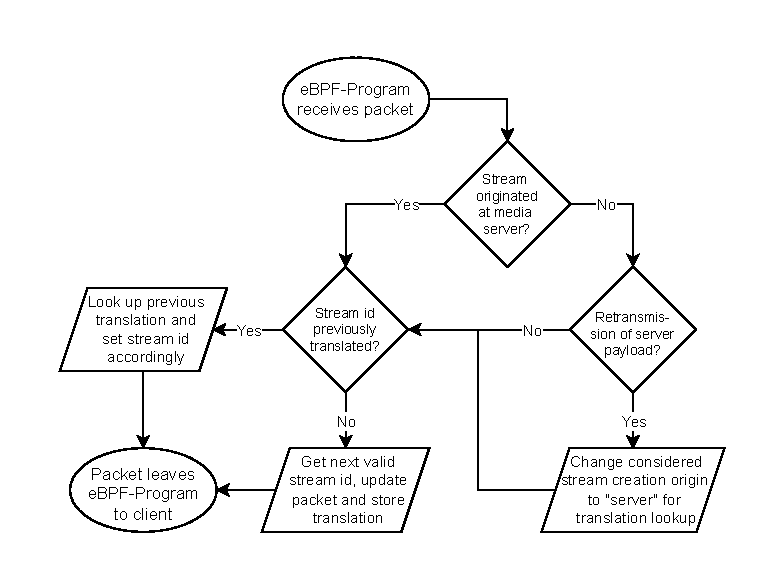
\includegraphics[width=0.7\textwidth]{figures/03_fast_relays/stream-id-translation.drawio.pdf}
    \caption[Stream id translation schematic]{Flow diagram of stream id translation process.}\label{fig:stream-id-translation}
\end{figure}
% Since the QUIC protocol works with packet numbers for a given connection it is necessary for 
% the egress program to make sure the forwarded packets together with the userspace packets
% provide a consistent state. 
% For this the egress program maintains its own packet number counter for each connection.
% That way only one counter has to be maintained and race conditions can be avoided.
The aforementioned packet number translation means that the packets sent by the userspace are 
likely to have a different packet number than the one chosen by the QUIC library.
This might lead to inconsistencies again when receiving acknowledgements but can be avoided by 
remembering the translation in a map as well as storing only packet-objects in the 
Go library that have the correct state.
This technique of ``storing'' a packet that the userspace either has sent itself or does not know
about since it comes from the media server will be referred to as ``packet registration''.
This initially gives a brief window where a packet was sent out but is not saved in the history
of the QUIC library but once the packet is then processed by the userspace routine handling the 
registration, any incoming ACKs for this packet can be processed correctly.
The next section will go more into detail on how the packet registration works.
Later we will also look at the implications of sending a packet the library does not know on 
retransmissions.
Even though the stream id translation works very similar to the packet number translation it 
does not have the need for any additional work after the packet has been sent out since our 
approach uses unidirectional streams only and thus the relay does not care about changes in 
the used stream id. % TODO: maybe reorder the sentences a little bit

\subsection{Packet Registration}
In order to make the congestion control algorithm that is running in userspace
usable we need to inform the QUIC library about the forwarded packets.
This again happens via BPF maps and a separate go routine that continuously
polls new entries in the map and processes them.
Entries are then added to the packet history to allow the receipt of ACKs.
Besides that, the congestion control algorithm will be informed about the
forwarded packet in order to be able to react to potential congestion events.
Figure~\ref{fig:forward-registration} visualizes the setup for this process.
\begin{figure}[H]
    \centering
    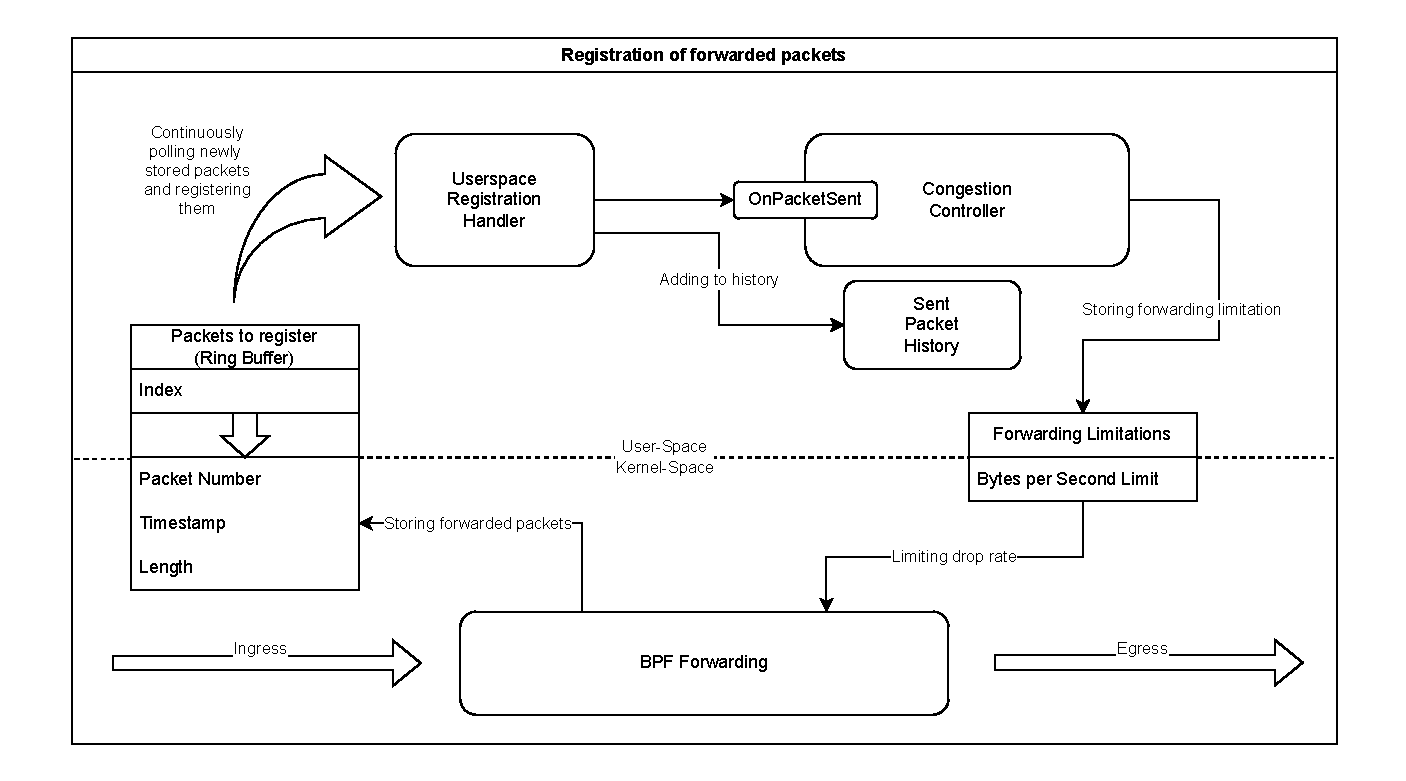
\includegraphics[width=0.7\textwidth]{figures/03_fast_relays/forward-registration.drawio.pdf}
    \caption[Packet registration schematic]{Internal setup for registering forwarded packets as well as incorporating forwarding
    limitations for the BPF program.}\label{fig:forward-registration}
\end{figure}

\subsection{Retransmissions of Forwarded Packets}
TODO

\section{Userspace Synchronization}\label{sec:userspace_synchronization}

Since one of the main ideas we propose is to avoid passing a packet all the way
through the network stack up to userspace at the relay, we create the 
problem that the application itself is not aware of packets that 
are being sent.
To conquer this issue, we suggest a setup that establishes communication
between the application- and the eBPF program.
To keep the improvement we gained by not passing packets to userspace during the 
critical path, this communication will happen in a delayed fashion, that is 
decoupled from the actual sending of media data.

The main resource we use for this communication will again be eBPF maps that
will contain information on the time a packet was sent together with protocol-specific 
data like packet-numbers or stream-identifiers (for both packet-number 
and stream-id the old and the new, i.e.~tranlsated, values will be stored).


% \subsection{User Space Avoidance}
% TODO 

\subsection{Subscription and State Management}
As already mentioned in~\autoref{sec:ebpf_setup}, an eBPF program handling incoming
traffic from the client will save client connection information like MAC address, IP 
address, et cetera, in a map for later access.
Also, an internal counter will give each client a unique identifier. % TODO: mention somewhere that this identifier has to be sequential and therefore does not support "unsubscribing" yet
With that, the only thing that happens in terms of communication between the application 
and the relay in case of a new subscription is that the application will update the 
\textit{number-of-clients} counter that is accessed by the eBPF program and used for packet duplication purposes.

Regarding stream state management, there is also little additional communication since the 
server is expected to use QUIC's unidirectional streams for sending the media data. 
That means the relay does not need to know about the stream details except if it 
has to trigger a retransmission.
% TODO: already mentioned
% If that is the case, the stream-id contained in the packet (meta-)data, that was read from the eBPF map, 
% will be used to manually create a stream with the correct id.
% It is important to manually set the correct id since the relay might not use the same id for the 
% next unidirectional stream it opens.
% Also, the client expects the retransmission to be sent on the same stream-id as the original packet
% since a retransmission happens within the same stream-context.

Since a client can also unsubscribe from a certain media stream, the relay needs to support
this as well.
This is done by simply decrementing the \textit{number-of-clients} counter and making sure the 
client ids stay in a usable state (i.e.~the relay is not duplicating packets for unsubscribed 
clients).
Our prototype implementation does not consider this yet, because our proof of concept and 
performance tests do not require it.

\subsection{Relay Caching}
Caching of data within a relay, which is required by the MoQ standard, is something we essentially get
for free since we are passing on an unaltered copy of any incoming packet from the server to the 
application at the same time we forward all the other packet copies to egress.
This means the application is able to receive any data from the server as if this was a normal connection and 
store, e.g.~the last \verb|n| second(s) worth of data in a cache.
Then, once a new connection is established, the relay could, in parallel to incrementing the kernel counter 
representing the number of clients, also send out cached data so that the client receives it
as early as possible.

One aspect that we still left open is the point in time when the relay should stop 
sending cached data since the forwarded data is up-to-date.
This also includes the question of how the client can handle potentially duplicate media data if the 
cached- and the forwarded data happen to overlap.
Such questions would likely require further experimenting and testing to find a good solution.

\section{Congestion Considerations}\label{sec:congestion_considerations}
QUIC, like many other modern transport protocols, contains congestion 
control mechanisms regulating the rate at which data is sent to a client.
This is primarily done to avoid the network becoming congested, but it also
has the secondary effect of circumventing the problem of overwhelming the client.
Simply forwarding all packets the relay receives from the server would cause 
the relay-client connection to no longer have its own congestion control.
Rather the rate at which the relay sends/forwards to the client would be determined
by the server's congestion control algorithm, i.e.~the network congestion between 
server and relay.
Obviously, this is not a desirable situation, so our approach suggests the eBPF 
program at egress to have its own congestion control functionality.

\subsection{Client Congestion}
Already hinted at in figure~\ref{fig:forward-registration}, it is shown that once a packet is 
registered, there will also be a map update that will be triggered by the congestion controller.
This map update will tell the eBPF egress program how much data it is allowed to send out. 
In figure~\ref{fig:forward-registration} this is visualized exemplary as ``Bytes per Second Limit''
but the idea is that both the function determining how limits and thresholds are calculated from 
the information on incoming packets as well as the actual handling within the egress program 
will be application-specific and defined by the relay engineer.
We experimented with approaches that use the QUIC internal measurements like the RTT, 
introduce new measurements like exponential-weighted moving averages, or even use an 
out-of-band connection where the relay expects direct feedback from the client.
All these possibilities show that there is a lot of room for experimentation and optimization
in this area.
This, however, will not be explored further in this thesis and is left for future work.
\\

\subsection{Packet Filtering and Dropping} % TODO: not sure if like this part
Assuming that the network congestion state is known and communicated to the relay, one can 
use the priority-information within a packet (that is expected to be set by the server) to
decide which packets should be forwarded and which ones should be dropped.
One difficulty in this approach is that the dropping mechanism essentially works as an online-
algorithm, meaning that it does not have full knowledge of the traffic, especially not of 
future packets.
This means that a case like the following could happen:
\begin{itemize}
    \item The traffic contains packets within the priority range of 1 to 5 (5 being the highest priority).
    \item Given the current network congestion to the client, the relay decides to drop 
            all packets below priority 3 as well as 50\% of the packets with priority 3.
    \item The remaining byte limit to be sent out is running low, and a packet with priority 3 
            comes in which is sent since the relay already dropped a lot of previous priority 3 packets.
    \item The next packet turns out to be a priority 5 packet which would overshoot the byte limit if sent.
\end{itemize}
In this example, one could use many different heuristics to handle the situation.
One could always keep enough byte limit left so that a high-priority packet can always be sent.
This, however, essentially just lowers the byte limit for all other packets while making it higher 
for high-priority packets.
Therefore an individual byte limit per priority could also be used right away.
Also, this approach might cause problems if a lot of high-priority packets come in at once, 
e.g.~in case of very ``bursty'' traffic.
Another way that could be used to handle this uncertain situation is to allow for temporary 
overflows of the byte limit.
This would make the limit more of a soft limit that can be exceeded for a short time.
However, this is another heuristic highly dependent on the specific use case and
traffic patterns, which is why we did not implement it in our prototype.
Overall we can say that implementation-wise it is not hard to drop packets, but the actual
difficulty lies in finding a reasonable way of deciding which packets to drop.
\section{Integration and Prototype}\label{sec:integration_and_prototype}
TODO

\subsection{Compatibility}
TODO

\subsection{Source Code Repositories}\label{sec:source_code_repos}
For the development of the relay and the eBPF programs, we have come up with the following repositories:
\begin{itemize}

    \item \textbf{Fast-Relay}~\parencite{adaptive-moq-repo}:
    This is the main repository providing the eBPF program implementations as well as examples of 
    server, relay and client implementations in Go.
    
    \item \textbf{Quic-Go Adaptation}~\parencite{quic-go-prio-packs-repo}:
    This repository is a fork of the QUIC library ``quic-go''~\parencite{quic-go-repo} and provides a 
    plain Go implementation of the QUIC protocol.
    For our thesis we needed to make some adaptations to the library to support some hook points for 
    separate functions which should be specifically designed to handle the underlying eBPF setup with its eBPF-Map usage. 
    
    \item \textbf{MoQ-Transport Adaptation}~\parencite{priority-moqtransport-repo}:
    This repository is a fork of the ``MoQ-Transport''~\parencite{draft-moqtransport} protocol repository and provides
    some needed adaptations to our examples. One such adaptation is that the server needs to support a 
    categorization of payloads into different priorities in order for the eBPF program to be able to 
    deliberalty drop packets in case of congestion.
    Getting these priorities could be as simple as differentiating only between I- and P-frames in a video 
    stream or more complex based on the needs of the application and the wanted granularity of the congestion 
    control.
    
\end{itemize}
